\chapter{Related work}

This chapter describes C\# type inference together with its injection into the Roslyn compiler.
Then we compare it with traditional Hindley-Milner type inference and it's variance in Rust language.
At the end, we present C\# issues presented on the Github repository which we use later to prioritize the improvement to make it more likely to be accepted by \ac{LDM}.

\section{C\# type inference}

\change{Type system(struct, class, and interface)}
\change{Inheritance}
\change{Overloading}
\change{Nullability analysis}
\change{Dynamic}
\change{Generics(struct, class, method, and interface)}
\change{Generics(where clauses, invariance, variance, and contra-variance)}
\change{Method type inference}
\change{var, target-typed new, target-typed ternary operator}

%We start with description of C\# type system and it's selected parts as a base for explanation the type inference.
%C\# is strongly typed language implicating that every value has a type.
%\par
%The fundamental characteristic of the type system is inheritance.
%We show an overview of inherited types in the following figure \ref{img01:typeSystem} to better describe it.
%\texttt{System.Object} is a base type which is inherited (directly or indirectly) by all other types.
%Types can be divided on reference and value types.
%Reference types consists of user defined classes (\texttt{class}), interfaces \texttt{interface}, \texttt{System.Object}, \texttt{System.Enum}, \texttt{System.ValueType} and other classes and interfaces from standard library.
%Two last mentioned classes are kind of special.
%Every type inheriting from them become a value type.
%Value types consists of user defined structures (\texttt{struct}), enums (\texttt{enum}), numeric types and other structures or enum from standard library.
%Since we are interested in type inference, we focus on difference between them in a compilation time.
%Classes can be inherited by other classes.
%Interfaces can be inherited by other interfaces and implemented by classes or structures.
%Structures can't be inherited.
%The next important characteristic for us is overloading.
%C\# types can contain multiple method definitions with the same name but different arguments.
%\par
%From C\# version 2.0, type system contains generics, enabling to reuse code.
%We can have a generic class, interface, struct, or method.
%Generics allow as to specify type parameters of the mentioned entities and work with them as real types.
%Providing type arguments to generic entities is called construction of generic entity.
%As an example of generic entity we can take \texttt{System.Collections.Generic.List<T>} representing resizeable array of \texttt{T}.
%Since we can assign any type to the type parameter, we can't use any methods, which doesn't have all types.
%This problem is solved by \texttt{where} clauses which restricts the type parameter by a constraint. 
%The most common constraint is common inherited class which extend allowed methods which can be called on the instance of the type parameter.
%\par
%\begin{figure}[b!]
%\centering
%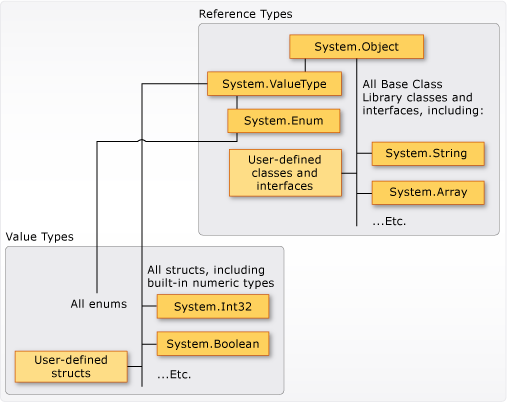
\includegraphics[width=140mm, height=100mm]{../img/value-reference-types-common-type-system}
%\caption{C\# type system \cite{online:cSharpTypeSystem}.}
%\label{img01:typeSystem}
%\end{figure}

\section{Roslyn}

\change{Overview of compilation pipeline}
\change{Binder}
\change{OverloadResolution}
\change{MethodTypeInferrer}
\change{NullableWalker}
\change{Dynamic biding vs. runtime binding}

\section{Hindley-Millner type inference}

\change{Hindley-Millner type system}
\change{Set of rules}
\change{Restriction and possible extensions}

\section{Rust type inference}

\change{Rust type system}
\change{Type inference context}
\change{Type inference across multiple statement}
\change{Constructor type inference}

\section{Github issues}

\change{Mention related Github issues and csharplang repo.}
\change{Roslyn and csharplang repo}
\change{Proposal champions}
\change{Related issues}
